\documentclass[10pt, a4paper]{ctexart}
\usepackage[margin=1in]{geometry}
\usepackage{bm}
\usepackage{amsmath}
\usepackage{graphicx}
\usepackage{float}
\usepackage{listings}
\usepackage{tikz}

\renewcommand{\figurename}{Figure.}
\renewcommand{\tablename}{Table.}

\begin{document}
\title{Assignment 3}
\date{}
\author{}
\maketitle

\section{A window into NER}
\begin{enumerate}
    \item {
        \begin{enumerate}
            \item Example sentences like "Ford is a good company" and "Benz invented cars", where "Ford" and "Benz" can either be a person and an organization.
            \item Using features helps us eliminate ambiguity.
            \item Features like whether the word is capitalized or whether the word is subjective.
        \end{enumerate}
    }
    \item {
        \begin{enumerate}
            \item If we use a window of size $w$, the dimension of $e^{(t)}$ will be $(2w+1)\times V$, the dimension of $W$ will be $D\times H$ and the dimension of $U$ will be $H\times C$
            \item Assuming that we usee a window of size $w$, then the computational complexity is: {
                \begin{align*}
                    O\big(T\times(2w+1)\times(V\times D+D\times H+H\times C)\big)
                \end{align*}}
        \end{enumerate}
    }
    \item {
        \begin{enumerate}
            \item See file q1\_window.py
            \item See file q1\_window.py
            \item See file ner\_model.py
        \end{enumerate}
    }
    \item {
        \begin{enumerate}
            \item The best development entity-level $F_1$ score is $0.83$, and the corresponding token-level confusion matrix is: {
                \begin{table}[H]
                    \centering
                    \begin{tabular}{c|c|c|c|c|c}
                        \hline
                        go$\backslash$gu&PER&ORG&LOC&MISC&O\\
                        \hline
                        PER&2942&54&59&16&78\\
                        ORG&134&1651&100&71&136\\
                        LOC&38&116&1865&25&51\\
                        MISC&34&61&40&1020&113\\
                        O&37&39&20&28&42635\\
                        \hline
                    \end{tabular}
                \end{table}
            } From the above confusion matrix we know that our model often confuses person's name with organization name, location name with organization name.
            \item One possible limitation of window-based model is the trade-off between window size and computational cost, in theory, the larger the window size is, the better our model is. However, large window size will also increase the computational cost, so in practice sometimes we have to balance between these two factos. Another limitation of window-based model is that is can only take local information into consideration. One drawback of these two limitations is that our model may not be able to take information that are far away from the current word into consideration. For example, when we type in the sentence "Ford is a good man", our model will predict "Ford" as an organization name, however, if our window size is big enough or our model can use all words rather than words in the window to do prediction, the model will see "Ford" is a "man", therefore will successfully predict it as a person's name.
        \end{enumerate}
    }
\end{enumerate}

\section{Recurrent neural nets for NER}
\begin{enumerate}
    \item {
        \begin{enumerate}
            \item The RNN model has an additional hidden-to-hidden matrix $W_e$, which has about $D\times H$ parameters.
            \item The computational complexity is: {
                \begin{align*}
                    O\big(T\times (V\times D+H\times H+D\times H+H\times C)\big)
                \end{align*}
            }
        \end{enumerate}
    }
    \item {
        \begin{enumerate}
            \item For example, say we have the sentence "Bob is a good man", and first our model predict every word in this sentence as {\bf{PER}}. If we then change our model to predict every word as {\bf{O}}, the cross-entropy cost will decrease, however, the $F_1$ score will decrease from $\frac{1}{3}$ to $0$.
            \item It is difficuly because $F_1$ score is non-convex.
        \end{enumerate}
    }
    \item See file q2\_rnn\_cell.py
    \item {
        \begin{enumerate}
            \item The loss will be larger and the gradient updates will converge slower. By using masking, we simply ignore the loss term corresponding to the padding token, therefore, the magnitude of loss and gradient will be the same as before.
            \item See file q2\_rnn.py
        \end{enumerate}
    }
    \item See file q2\_rnn.py
    \item See result in folder results/
    \item {
        \begin{enumerate}
            \item One limitation is that this RNN model makes decision at every position using only information before the current word, and don't take words afterwards into consideration. Examples like "Ford is a good man", the word "Ford" here got misclassified as {\bf{ORG}}, which was supposed to be a {\bf{PER}}. Another limitation is that this RNN model will gradually loss information about words appeared at the beginning as it go through the whole sentence. One example is "As a good student, all teachers in school like Ford." where "Ford" was misclassified as {\bf{LOC}}.
            \item For the first limitation, we can modify the structure of this RNN model and let it iterate through the whole sentence first, and then use the computed hidden state to make decisions for each word. For the second limitation, we can use more advanced RNN like LSTM.
        \end{enumerate}
    }
\end{enumerate}

\section{Grooving with GRUs}
\begin{enumerate}
    \item {
        \begin{enumerate}
            \item Let $b_n=-1,~W_h=2,~U_h=2$
            \item Let $W_z=-1,~U_z=1,~W_h=1,~U_h=0$
        \end{enumerate}
    }
    \item {
        \begin{enumerate}
            \item Assuming that such 1D RNN do exist, and then we have: {
                \begin{align*}
                    \left\{
                        \begin{matrix}
                            W_h+b_h>0\\
                            b_h\le 0\\
                            W_h+U_h+b_h\le 0\\
                            U_h+b_h>0\\
                        \end{matrix}
                        \right.
                \end{align*}
                } So we have $W_h>0$ and $W_h<0$ at the same time, which is a contradiction. Therefore, there do not exist such 1D RNN.
            \item Let $U_z=1,~W_z=-1,~W_h=1,~b_r=1,~U_h=-1$
        \end{enumerate}
    }
    \item See file q3\_gru\_cell.py
    \item See file q3\_gru.py. The learning dynamics are listed as follows: {
        \begin{figure}[H]
            \centering
            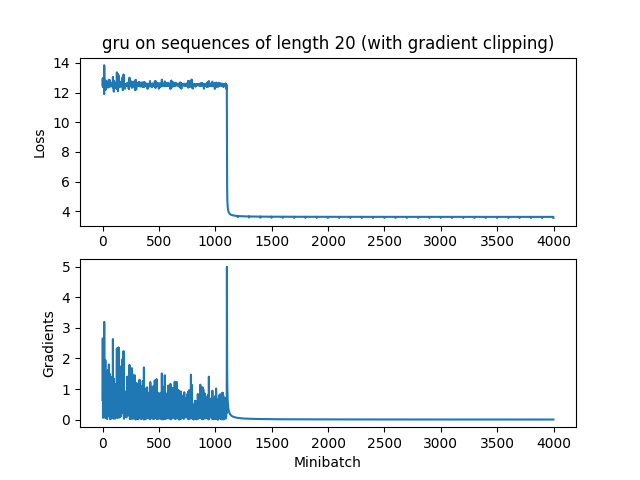
\includegraphics[width=0.7\linewidth]{../q3-clip-gru.png}
            \caption{GRU-clip}
        \end{figure}
        \begin{figure}[H]
            \centering
            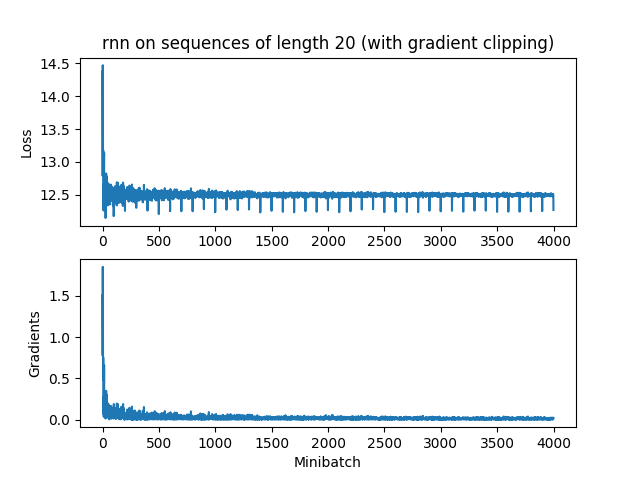
\includegraphics[width=0.7\linewidth]{../q3-clip-rnn.png}
            \caption{RNN-clip}
        \end{figure}
        \begin{figure}[H]
            \centering
            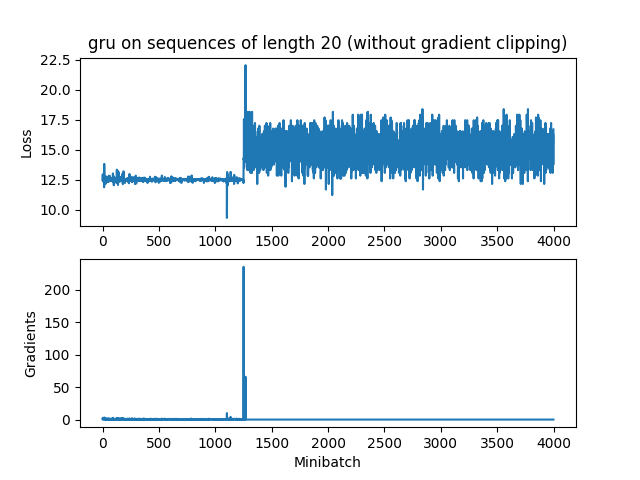
\includegraphics[width=0.7\linewidth]{../q3-noclip-gru.png}
            \caption{GRU-no-clip}
        \end{figure}
        \begin{figure}[H]
            \centering
            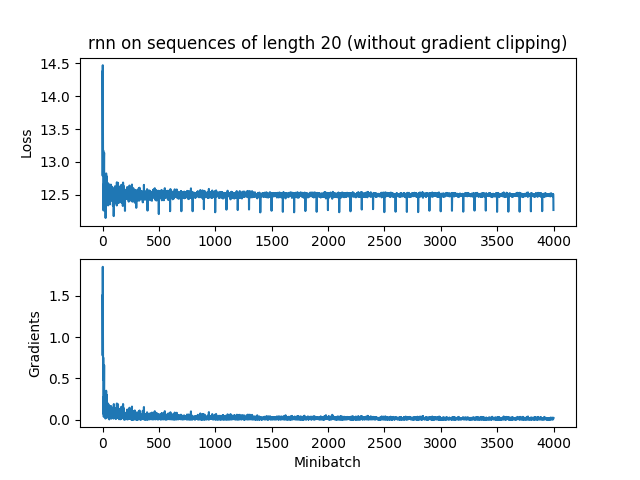
\includegraphics[width=0.7\linewidth]{../q3-noclip-rnn.png}
            \caption{RNN-no-clip}
        \end{figure}
    }
    \item {
        \begin{enumerate}
            \item RNN suffers vanishing gradient and GRU suffers exploding gradient. Gradient clip helps GRU with exploding gradient problem.
            \item GRU does better, this might because it suffers vanishing gradient problem less and therefore can have more information to update the model and achieves a better optimal point.
        \end{enumerate}
    }
    \item See result in folder results/
\end{enumerate}
\end{document}